\documentclass[twocolumn]{article}
\usepackage[utf8]{inputenc}
\usepackage[english]{babel}
\usepackage{abstract}
\usepackage{booktabs}

\usepackage{siunitx}    
\usepackage{makecell}


\usepackage{graphicx}
\graphicspath{ {latexIMG/} }


\title{AML Project
\\Federated Learning: where machine learning \\and data privacy can coexist
}

\author{
Alfredo Baldó Chamorro | 
Basiten Bartholom |
Giuseppe Salvi
}
\date{February 2022}

\begin{document}

\maketitle

\section{Abstract}
With the mass of data generated each day by multiple sources (i.e. IoT), machine learning has a bright future. Unfortunately, a huge part of these data are not usable due to their private nature regarding the users. Federated learning is a machine learning framework aiming to guarantee this privacy by keeping the data locally on the device (i.e. mobile phones).
\section{Introduction} %mandatory

Introduced by Google in 2016 [1] \emph{https://arxiv.org/abs/1610.05492}, Federated Learning enables models to be iteratively trained in a decentralized way, on the local devices. At each round, a subset of sources (also called \emph{clients}) are selected to perform local training on their own data. Then, the centralized model aggregate the ensemble of updates to make the new global model and send back it to another subset of clients. 

As a part of our Advanced Machine Learning course at Politecnico di Torino, this paper will cover our work on the replication of the experiment proposed by [2] \emph{https://arxiv.org/abs/2003.08082} on the CIFAR10 dataset [3] \emph{https://www.cs.toronto.edu/~kriz/cifar.html} which consists of analyzing the effects that client's data distributions have on federated models. Especially distributions such as Non-Identical Class Distribution, meaning that each client have a different class distribution and Imbalanced Client Sizes, meaning that each client have a different amount of data. 

We will cover the federated scenario using the standard FedAvg aglorithm with multiple sets of parameters and evaluate the one performing best. We will experiment different settings such as data distribution, normalization layers and group normalization. Moreover, we will propose and test a solution in order to solve one of the identified problems.

\section{Related Work} %mandatory
This experiment has already been performed by \emph{Tzu-Ming Harry Jsu et al.}[2]  on the iNaturalist-2017 [4] \emph{https://paperswithcode.com/dataset/inaturalist} dataset.. They provided an analyze of the effect of learning with per-used data and proposed two new algorithms (FedVC, FedIR) and provided new large-scale datasets with per-user data.

A different algorithm (FedAvgM) has been proposed by \emph{Tzu-Ming Harry Jsu et al.}[5] \emph{https://arxiv.org/abs/1909.06335} using momentum on top of SGD to accelerate the network training. This approach changes the way the weights are updated to add momentum at the server.

\section{Methods} %mandatory describe algorithms
There are various steps in the building of the final algorithm. In this section we will explain the decisions that led us to choose the values for the parameters and our choice for different algorithms implemented. 

Federated learning applied in the real world, would take into account multiple devices with different characteristics (CPU capacity and speed...). The model and algorithm selection was chosen on the basis of a hypothetical implementation on different devices.  

\subsection{Problem setup}
Federated Learning consists of a client and a server side. Considering the CIFAR10 dataset contains 50 000 samples for training and 10 000 samples for testing, we thought that choosing the number of clients K = 100 would be representing a real-world case (averaging 500 images per client for training). 

Moreover, in order to simulate real world data, we implemented into the code a variability Delta regarding the distribution of the data among clients. The variable added some randomness to the quantity of data that each client would be seeing. For example, if Delta = 100, each of the 100 clients would have a minimum of 400 images and a maximum of 600. (50 000 / 100 = 500 +- 100).


To add up, the distribution of data was considered to be performed randomly. The variability Delta introduced was not great, and this was done intentionally. The problem of some client having way bigger amount of images (2-3 times) than others could have been solved with the creation of additional virtual clients and splitting the data among them. In terms of implementation this would be equal to increasing the number of clients from K to K + i, where i is the number of the virtual clients created (CHECK IF IT MAKES SENSE) 

Finally the number of selected clients C, was chosen based on performance (INSERT TABLE OR GRAPHIC). In fact, with a C <0.3 the performance decreased significantly (put some values).
INSERT GRAPHICS BETWEEN DIFFERENT C AND THE CONSOLIDATED MODEL

\subsection{Network}

With that in mind, for the neural network we chose a variation of LeNet5 which has two 5×5, 64-channel convolution layers, each precedes a 2×2 max-pooling layer, followed by two fully-connected layers with 384 and 192 channels respectively and finally a softmax linear classifier (REFERENCE TO PAPER 3 an insert image if possible). 

As each device implements our model and considering each having a different computational capacity, we chose a small and simple network in order for the computation to be the quickest possible but also having the capacity to gather information from the client's dataset.

\subsection{Algorithm}
Regarding the server aggregation we chose to go with the Federated Average algorithm (FedAvg). The FedAvg (PUT FORMULA AND REFERENCES) consists on aggregating the weights of the clients according the number of images each client sees, with respect to the total number of images of the dataset.(SPECIFIY MORE AND CORRECT)
The FedAvg algorithm is simple, but useful enough in order to get an acceptable accuracy.

In addition, we also considered a variant of the Federated Average algorithm with server momentum, called FedAvgM [REFERENCE PAPER]. Vanilla FedAvg updates the weights via (FORMULA). To add momentum at the server, we compute instead (FORMULA) and update the model with (FORMULA). 
We wanted to make a comparison between the two algorithms and see what impact the introduction of the momentum server had on the rapidity of convergence and oscillations, particularly in the scenario where clients have different data distributions


\section{Experiments} % mandatory
\subsection{Federated Average}
As baseline model, Federated Average (FedAvg) algorithm was chosen. In order to get an idea of the performance of the algorithm, a comparison with the centralised model was needed. 

First of all, we needed to fine-tune the parameters for the centralized model. We decided to adopt the number of epochs E = 100, as a compromise between performance and computational cost. We discovered as best learning rate the value LR = 2e-3, because lower values had worse results, while higher values showed overfitting. With that in mind, in the federated model, we used the same learning rate and decided to use 20 rounds of 5 local epochs, to have a fair comparison between the two scenarios.
(ADD A COUPLE OF PLOTS FOR CENTRALISED MODEL FINE-TUNING)

Figure \ref{AccCompFedCent} represents the difference in performance between centralised and federated model. The figure represent a comparison between the two models while changing parameters in the configuration. It's evident and as awaited, that the centralised model has a better performance. The FedAvg does not lead to a good accuracy (hardly reaching 70\%). Still, being a model without any further optimization, the accuracy was thought as acceptable. (ADD TAGS TO COLUMNS a,b,c and explain the details below)


\begin{figure}
    \centering
    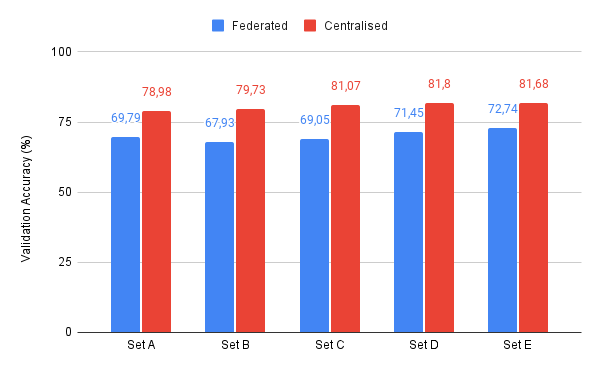
\includegraphics[width=0.5\textwidth,height=.3\textheight]{FedAccuracyComp.png}
    \caption{Accuracy comparison between centralised and federated model}
     \label{AccCompFedCent} 
\end{figure}
\subsection{Group and Batch Normalization}
In order to be able to decide which model implementation is better, a comparison between normalization was made in table \ref{batchNormComp}. What can be extracted form this experiment is that normalization is relevant for the accuracy. It's true that the accuracy does not improve much in the centralised model by adding normalization (from 79,73 to 81,7 \% for no normlization and group normalization respectively). However, in the federated learning, normalization seems crucial, as the worst performance was achieved by the model without it (65\%). Moreover adding the normalization layer, added up to 9\% in accuracy performance. 


\begin{table}
\centering
\begin{tabular}{||c c c||} 
  \toprule
 \makecell{Model} & \makecell{Validation Accuracy (\%)} & \makecell{Normalization}  \\
  \midrule
  Federated  & 73,45 & Batch \\
 \hline
 Federated & 65,49 & No\\
 \hline
  Federated &  \ensuremath{\mathbf{74,57}} & Group\\
 \hline
  Centralised & 78,98 & Batch\\
   \hline
  Centralised  & 79,73 & No\\
   \hline
  Centralised  & \ensuremath{\mathbf{81,7}} & Group\\
  \bottomrule                             
\end{tabular}
\label{batchNormComp}
\caption{Performance comparison with batch normalization}
\end{table}


\subsection{Different data sizes}
In order to simulate different quantity of data that each client is going to have, a variable Delta was implemented in order to add randomness. The experiment was followed by changing the number of groups division of the group normalization layer 1 and 2. The results are represented in figure \ref{AccDiff}, illustrating with different group normalization parameters, the accuracy over the validation set. 

Sticking with figure \ref{AccDiff}, over 8 tests done, three performed better with the Delta variable activated, and one specifically (8-2) outperformed every over scenario with an accuracy of 78,27\%. The accuracies presented in the figure \ref{AccDiff} are very similar between each other, even though with the deactivation of the Delta variable (each client with the same amount of data) it seems to perform better, as 5/8 tests had greater accuracy than with using Delta.

(CHECK THAT AGAIN, THIS COULD BE MISLEADING)
However, computing the mean of the performances, we get 72,1 \% and 72,8\% for no Delta and Delta respectively. This translates to the fact that even though the Delta variable presented better accuracy, the accuracy achieved with the Delta activated is greater. This results could be explained by the fact that adding some randomness to the data quantities helps the prediction of classes.
(DO TWO OR THREE EXPERIMENTS WITH DIFFERENT DELTA)

\begin{figure}
    \centering
    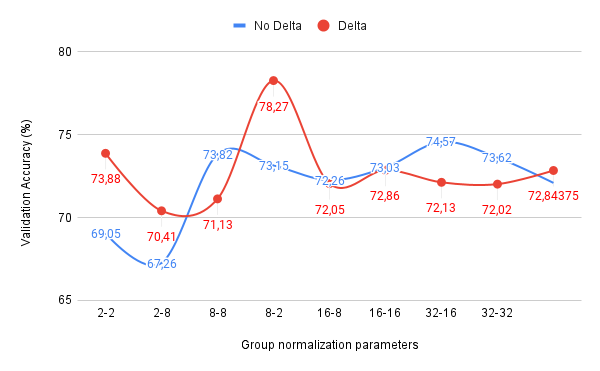
\includegraphics[width=0.5\textwidth,height=.3\textheight]{groupnormalizationDeltaNoDelta.png}
    \caption{Accuracy over validation set with Diff variable activated or not}
     \label{AccDiff} 
\end{figure}

\subsection{Dirichlet distribution}

Regarding implementation, in order to achieve a better understanding of the possible accuracy outcomes, taking into account different data distribution is crucial. \textbf{\emph{NOTE : Not sure to understand the previous sentence.}} In order to simulate client getting different data distribution, we used the Dirichlet distribution. The parameter Alpha, represents how different the distribution is between clients: with a greater Alpha, the distributions 
would be similar, with smaller Alpha, the distribution between clients differs.
In particular, when Alpha is equal to 0 each client has access to data belonging to only one class.
(1)
(ADD GRAPHS WITH DIRICHLET DATA DIVIDED)
In order to implement it, we used data already distributed with different Alpha parameters, taken from (PUT REFERENCE TO GIT REPO).


We used the already splited data from [x] \emph{https://github.com/google-research/google-research/tree/master/federated_vision_datasets} where the Alpha goes from 0 to 100 for the CIFAR10 dataset.


The results are shown in figure \ref{AccAlpha}. This image clearly illustrates the fact that expanding the difference in the dataset distribution between clients (lower Alpha), as expected, leads to the decrease in accuracy. 
Moreover, from the plots of training and validation accuracy, we see how the lower alpha is, the higher is the number of oscillations.
The accuracy on the training is higher because the smaller the Alpha, the smaller the number of classes each clients gets, hence a perfect prediction is expected. 
(EXPAND THESE THOUGHTS A BIT, ADD AT LEAST THREE PLOTS FOR ACCURACY ex: a=1,10,100)
(2A, 2B, 2C)

To obtain results that are more similar to the iid scenario also for lower values of alpha we need to increase a lot the number of communication rounds. For example, in Figure 10 (INSERT FIGURE WITH 200 rounds WITH alpha = 1) validation accuracy reaches around 65\% accuracy like in the iid setting.
(3)

Finally, the figure \ref{AccAlpha} states that the group normalization model over-performs the model without normalization. This behavior goes along with the results gotten in the normalization experiments, and in this situation, normalization has an even more important role. (MAYBE WRITE A LITTLE MORE).
.


\begin{figure}
    \centering
    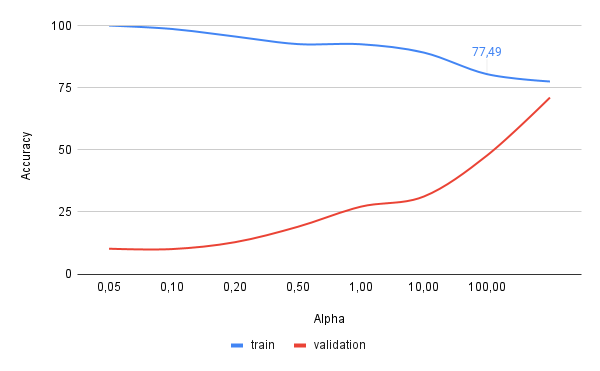
\includegraphics[width=0.5\textwidth,height=.3\textheight]{alphaAccuracy.png}
    \caption{Accuracy over different values of Alpha}
    \label{AccAlpha} 
\end{figure}


\subsection{Federated Average Momentum (additional contribution?)}
We start analyzing the results with the same setup of the previous experiments (Rounds = 20, Epochs = 5, Local Batch size = 32, K = 100, C = 0.3).
For the FedAvgM we used the same settings as in [REFERENCE FOR PAPER]: SGD as the optimizer for the server model,  momentum (beta) = 0.9, and centralised model learning rate fixed to 1.
From the accuracy and loss plots with iid data distributions for the clients, we can see how the results are very similar. However, the solution with server momentum has smaller oscillations and converges slightly faster. 
(4A, 4B, 4a, 4b)

We tried to see if for different values of momentum the behaviour changed. The plots of accuracies in figures (PLOTS of accuracy WITH 0.997 and 0.7) show that when beta is lower the number of oscillations is higher, and their height is bigger.
(5A, 5B)

With the non-iid data distributions for the clients, the results are slightly better than vanilla FedAvg's ones (SEE PLOT SIMILAR THAN PREVIOUS ONE). 
(ASK ALFREDO 6)
However, even in this case, there is a large presence of oscillations, particularly for small values of alpha, which makes comparison difficult.
(COUPLE OF PLOTS OF ACCURACY, SEE IF CONVERGENCE IS FASTER, IN THAT CASE ADD A COMMENT, MAKE A COMPARISON WITH PREVIOUS ONE IF SOMETHING CHANGES)
(7A, 7B, 7C)

Since in our original setting the number of rounds is too low to appreciate any major difference between the vanilla FedAvg and FedAvgM behaviors, we decided to change our setup by increasing the number of rounds to 1000, and decreasing the number of local epochs to 1 so that the computation could still be handled by our systems.
Our idea was to explore different regions of the Figure (FIGURE 5 FROM PAPER) from (LINK OF PAPER) to see if also in our setting we found the same behavior.
(8)
In the case with alpha = 1 both the models reached accuracy around 0.7 and their trend is very similar, with wide oscillations in particular at the beginning.
(9A, 9B)

Then we tried to pick a case in the rightmost part of Figure 5 (FIGURE FROM PAPER AS ABOVE) where the differences should be more evident, also changing the percentage of selected clients at each round (C) from 0.3 to 0.1. 
However, even on this occasion, the two algorithms achieve similar results. In this case FedAvgM's algorithm fails to achieve the expected accuracy. Probably with such low values of alpha it would take an even greater number of rounds, which we are not able to test due to the limitations of the hardware at our disposal. The major difference between the two plots is at the beginning, where FedAvg starts with a higher value of training accuracy and converges faster.
(10A, 10B)



\subsection{Conclusion}
SUM UP RESULTS AND 
\subsection{References}


\end{document}
